\section{Pipeline overview}
\label{sec:pipeline-overview}

\begin{figure}[!htb]
\centering
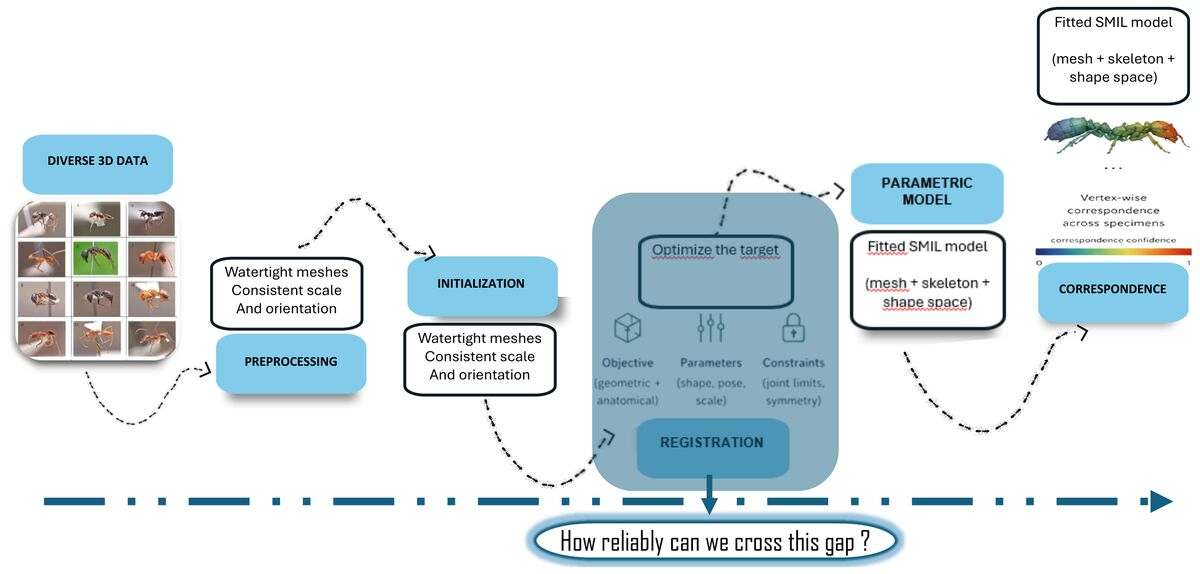
\includegraphics[width=0.78\linewidth]{figures/fig_pipeline_full.jpg}
\caption{The registration pipeline, from diverse raw scan data to a fitted
parametric model with explicit vertex-wise correspondence. The pipeline
stages are described in \S\ref{sec:preprocessing}--\S\ref{sec:registration};
the correspondence stage did not exist before this internship and is the
subject of Chapters~\ref{ch:diagnostics}--\ref{ch:validation}.}
\label{fig:pipeline}
\end{figure}

The delivered pipeline (Figure~\ref{fig:pipeline}) has four stages: preprocessing,
initialisation, registration, and, newly introduced during this
internship, an explicit correspondence-audit stage that reports, for a
fitted specimen, how confidently each vertex's identity can be trusted rather
than only how close the surfaces are. The following sections take each stage
in turn.
